%!TEX root = ../../thesis.tex
Traditional robots are made from rigid and dense materials that ensure accurate and repeatable motions. While rigid robotics excel at fast and precise motion, their structural rigidity lacks the compliance and mechanical robustness needed for safe and passive interaction in an unknown environment. Soft robotics, on the other hand, aim to improve the motion complexity and environmental robustness that is generally lacking its rigid counterpart. To further promote these topics in robotics, researchers aim to mimic living creatures by developing bio-inspired robots with similar morphologies and mechanical properties \cite{Falkenhahn2015,Suzumori1991,Godage2015,Godage2016,Marchese2014,Kriegman2019}.
The hyper-flexible and continuum-bodied structure in soft robots provides them with a rich family of motion primitives. Besides bio-mimicry, soft robotics has proven to be a prominent alternative for rigid robotics with a variety of applications, \eg, manipulation and adaptive grasping \cite{Galloway2016}, untethered locomotion and exploration through uncertain environments \cite{Marchese2014,Choi2011,Pilz2020}, rehabilitation \cite{Polygerinos2015}, and even minimal-invasive surgery \cite{Li2017a,Cianchetti2014}. Although the popularity of the field has increased exponentially in recent years, one of the first soft robots dates back already to the early 1990s, \eg, the work of Suzumori et al. (1991, \cite{Suzumori1991}). Yet, despite years of soft robotics research, their intrinsic hyper-flexible nature still possesses numerous challenges on modeling and control.

One major challenge in modeling is that the soft robot's elastic body undergoes large, continuous deformation. Since its inception, numerous works have addressed the kinematics for soft continuum robots \cite{Jones2006,Mochiyama1999,Mochiyama2003}; yet, its original framework stems from hyper-redundant robotics nearly a decade earlier \cite{Chirikjian1994}. Similar to soft robots, hyper-redundant robots exploit their high joint redundancy to achieve a broader range of tasks (\eg, shape control and collision avoidance) besides end-effector manipulation. To some extent, soft robots can be seen as the successor to hyper-redundant robots in which rigid mechanical joints or links are substituted with hyper-flexible soft elements. As a result, their dynamics involve a continuously deformable inertial body rather than the classical notion of rigid bodies. As such, conventional modeling approaches cannot be applied directly to these continuously deformable robots, stressing the importance of novel modeling strategies. In this respect, the dynamics of a continuously deformable soft robot are, in theory, of an infinite-dimensional nature. This paradigm shift has further emphasized the challenges in control-oriented modeling of soft robots, as their physical description are often more suited for a Partial-Differential Equations (PDEs) rather than Ordinary Differential Equations (ODEs).

Recently, some significant steps have been made toward formulating reduced-order ODE models for elastic continuum soft robots, paving a path toward model-based controllers. Perhaps one of the most popular techniques of spatial reduction is the so-called \textit{"Piece-wise Constant Curvature"} model or PCC for short. The PCC model assumes that a soft robot's reachability can be described using a number of spatially-constant curves, which are parameterized using a minimal set of generalized coordinates. Although PCC models can be seen as a significant oversimplification of true continuum mechanics at hand, these models have proven to be remarkably viable for various control applications. Besides its use in inverse kinematic control \cite{Marchese2014,Marchese2016,Jones2006}, PCC models have also shown to be suitable for feedforward controllers as demonstrated by Falkenhahn et al. (2015, \cite{Falkenhahn2015}); and more recently, closed-loop feedback controllers by Della Santina et al. (2019-2020, \cite{DellaSantina2020,Katzschmann2019}). Although the aforementioned works utilize the lumped-mass description, others have employed PCC models with uniform mass distribution \cite{Renda2018,Godage2015,Godage2016,Tatlicioglu2007,Tatlicioglu2007a} and current models even extend beyond the constant curvature \cite{Mochiyama2003,Chirikjian1994,DellaSantina2020}. However, in the face of significant external loading or (distributed) contact with the environment, the PCC assumption is relatively conservative and leads to undesired kinematic constraints on the continuum deformation. Besides, these models often need additional identification to model compliance as they do not originate from a continuum mechanical framework.

On the other hand, Finite-Element Method (FEM) models do originate from continuum mechanics and, due to their PDE description, provide a more accurate representation of deformations; and are particularly suited to deal with geometric and material nonlinearities. Duriez et al. (2013, \cite{Duriez2013}) and related works \cite{Coevoet2017,Largilliere2015,Goury2018} showed that reduced-order FEM models could play an important role in closed-loop control -- allowing accurate volumetric deformation and hyper-elastic behavior. Although such real-time simulations for FEM-based models are possible, a significant state-reduction is required to ensure sufficient computational speed. In the process, FEM-based models often lose desirable control properties, \eg, passivity preservation, which might play an important role in control. An alternative modeling strategy is the recently emerging geometrically-exact Cosserat-beam model. Similar to the PCC models, the Cosserat models have the merit benefit that they can be structured into a standard Lagrangian form -- the basis for robotics control theory. Rooted in a geometric method for describing the continuum mechanics using Lie theory proposed by Simo et al. (1986, \cite{Simo1986}), Boyer et al. (2021, \cite{Boyer2010, Boyer2021}) proposed a geometrically-exact modeling framework for Cosserat beams using nonlinear parametrization of the strain field. Other examples include the work of Renda et al. (2018, \cite{Renda2018,Renda2020}), providing various options for Piecewise-Constant Strain (PCS) and Variable Strain modeling approaches. Although recent variants of the Cosserat models offer good computational performance \cite{Till2019,Grazioso2019}, its use in model-based control is slowly upcoming.

In this respect, the topic of reduced-order modeling of soft robots is an active area of research. Yet, a challenge that is frequently overlooked in control-orientated research is the anisotropic material behavior, mechanical saturation, and more importantly, the nonlinear and possibly time-varying nature of the highly hyper-elastic soft materials \cite{Falkenhahn2015, Mochiyama2003, Till2019, Tatlicioglu2007}. This is further amplified by the fact that soft robots are known for their diversity in elastic materials and corresponding morphologies. Mustaza et al. (2019, \cite{Mustaza2019}) proposed a modified nonlinear Kelvin-Voigt material model to embody the complex material behavior of silicone-composite manipulators (so-called STIFF-FLOP actuators). A similar silicone composite actuator was experimentally validated by Sadati et al. (2020, \cite{Sadati2020}) who proposed a novel modeling approach with an appendage-dependent Hookean model and viscous power-law to describe nonlinear and time-dependent material effects, respectively. Both nonlinear material models show good correspondence with physical soft robots under various dynamic conditions, yet they lack general transferability to the soft robots with different geometries -- intrinsically captured by FEM-driven models. As of today, there are few control-oriented models that both offer geometry and material versatilely similar to FEM models and the control convenience similar to spatial curve models.

Ultimately, the strong nonlinearities paired with its continuous nature encourage the use of model-based controllers. Nevertheless, regarding the aforementioned model-based control approaches \cite{DellaSantina2020,Katzschmann2019,Falkenhahn2015}, the stability and performance of the closed-loop system could be undermined by uncertainties in physical parameters or unmodelled dynamics. Particularly for state-feedback linearization (e.g., inverse dynamic), as the inversion of inaccurately estimated systems could lead to poor performance and even instability. Adaptive control \cite{Slotine1988,Morgan1977} or energy-based controllers \cite{Ortega1998} might offer the needed robustness towards material uncertainties and unmodelled dynamics. Unfortunately, up till now, the applicability of adaptive and energy-based control techniques on soft robotics is scarcely explored. Franco et al. (2020, \cite{Franco2020}) used an adaptive energy-based controller that compensates for external disturbances on the end-effector, yet this controller can be extended to include various slowly-varying material uncertainties, \eg, hyper-elasticity and viscosity.

The contributions of the work are two-fold. First, to derive a finite-dimensional dynamic model of a continuum soft robot, where we briefly recapitulate existing modeling techniques for soft robot manipulators. To address the issue of infinite-dimensionality, we explore the PCC condition that allows for a low-dimensional description of the continuum dynamics. Although such modeling approaches have been thoroughly developed, we will address two issues that will aid the development of model-based controllers. We aim to bridge the gap between the PCC model and the underlying continuum mechanics by matching the quasi-static behavior to a Finite-Element-driven model (FEM), and we propose a reduced-order integration scheme using Matrix-Differential Equations (MDEs) to compute the spatio-temporal dynamics in real-time. Preliminary results of this work were shown in Caasenbrood et al. (2020, \cite{Caasenbrood2020}) and in Caasenbrood et al. (2022, \cite{}).
%

Second, in regards to the FEM-based hyper-elastic modeling and the possible presence of unmodelled dynamics (e.g., material uncertainties or external loads on the end-effector), a passivity-based adaptive controller is proposed that enhances robustness towards material uncertainties and unmodelled dynamics in closed-loop, slowly improving their estimates online. All source code is made publicly available at Caasenbrood et al. (2020, \cite{SorotokiCode}).%\highlight{(see the open software repository)}

\section{System development}
By using additive manufacturing, we developed a soft and flexible robot manipulator that is suitable for pick-and-place applications. The 3-DOF soft robot can be seen in Figure \ref{fig:C2:soft_robot}. The soft robot manipulator in this work is loosely inspired by the elephant whose trunk-appendage consists mainly of parallel muscles without skeletal support. The anatomy of the elephant's trunk provides an excellent study case, as they naturally exhibit continuum-body bending and moderate elongation \cite{Falkenhahn2015,Jones2006,Tatlicioglu2007}. Similar to the earlier soft robotic designs
\cite{Suzumori1991,Falkenhahn2015}, the developed soft robot can undergo three-dimensional movement by inflation or deflation of embedded pneumatic bellow network. The pneumatic network has three unique inputs, which labeled $\uB = (u_1,\,u_2,\,u_3)^\top$. By varying the input $\uB$, the soft robot can achieve bending in any preferred direction by differential pressurization of each channel ($<$0.1 \si{\mega \pascal}), \eg, $u_1 > u_2 = u_3 > 0$. Whereas, simultaneous pressurization accomplishes moderate elongation, \ie, $u_1 = u_2 = u_3$. As a demonstration, we provided the following pressure inputs to the system:
%
\begin{align}
  u_i(t) = \begin{cases}
          \;\;\erf(t)\cdot \left[P_0 - P_a\sin\left(\pi t + \delta\right)\right] \quad\;\; \textrm{for}\;\; i = 1,2 \\[0.35em]
          \;\;\erf(t)\cdot \left[P_0 - P_a\sin\left(\pi t \right)\right] \quad\quad\quad\;\; \textrm{otherwise}\;\ \\
           \end{cases}
\end{align}
%
where $P_0 = 5$ \si{\kilo \pascal}, $P_a = 15$ \si{\kilo \pascal}, $\delta = \frac{\pi}{2}$, and $\textrm{erf}(t) := \frac{2}{\pi}\int_0^\tau \exp(-\tau^2) \; d\tau$   the error function to ensure a smooth transient. The demonstration is shown in Figure \ref{fig:C2:soft_robot}.

%
\begin{figure}[!h]
 \vspace{-3mm}
  \centering
  \ifx\printFigures\undefined
  \else
  % This file was created by matlab2tikz.
%
\begin{tikzpicture}

\begin{axis}[%
width=0.712\textwidth,
height=0.249\textwidth,
at={(0.11\textwidth,0\textwidth)},
scale only axis,
xmin=0,
xmax=1,
ymin=0,
ymax=1,
axis line style={draw=none},
ticks=none,
axis x line*=bottom,
axis y line*=left,
colorbar style={width=6,xshift=-7.5pt}
]
\end{axis}

\begin{axis}[%
width=0.204\textwidth,
height=0.204\textwidth,
at={(0\textwidth,0.031\textwidth)},
scale only axis,
axis on top,
xmin=0.5,
xmax=796.5,
tick align=outside,
y dir=reverse,
ymin=0.5,
ymax=796.5,
axis line style={draw=none},
ticks=none,
colorbar style={width=6,xshift=-7.5pt}
]
\addplot [forget plot] graphics [xmin=0.5, xmax=796.5, ymin=0.5, ymax=796.5] {fig_C2_srm_example-1.png};
\end{axis}

\begin{axis}[%
width=0.204\textwidth,
height=0.204\textwidth,
at={(0.232\textwidth,0.031\textwidth)},
scale only axis,
axis on top,
xmin=0.5,
xmax=796.5,
tick align=outside,
y dir=reverse,
ymin=0.5,
ymax=796.5,
axis line style={draw=none},
ticks=none,
colorbar style={width=6,xshift=-7.5pt}
]
\addplot [forget plot] graphics [xmin=0.5, xmax=796.5, ymin=0.5, ymax=796.5] {fig_C2_srm_example-2.png};
\end{axis}

\begin{axis}[%
width=0.204\textwidth,
height=0.204\textwidth,
at={(0.464\textwidth,0.031\textwidth)},
scale only axis,
axis on top,
xmin=0.5,
xmax=796.5,
tick align=outside,
y dir=reverse,
ymin=0.5,
ymax=796.5,
axis line style={draw=none},
ticks=none,
colorbar style={width=6,xshift=-7.5pt}
]
\addplot [forget plot] graphics [xmin=0.5, xmax=796.5, ymin=0.5, ymax=796.5] {fig_C2_srm_example-3.png};
\end{axis}

\begin{axis}[%
width=0.204\textwidth,
height=0.205\textwidth,
at={(0.696\textwidth,0.03\textwidth)},
scale only axis,
axis on top,
xmin=0,
xmax=796.5,
xtick={0,500},
xticklabels={\empty},
tick align=outside,
y dir=reverse,
ymin=0,
ymax=800,
ytick={0,200,400,600,800},
yticklabels={\empty},
axis line style={draw=none},
ticks=none,
axis x line*=bottom,
axis y line*=left,
colorbar style={width=6,xshift=-7.5pt}
]
\addplot [forget plot] graphics [xmin=0.5, xmax=796.5, ymin=0.5, ymax=796.5] {fig_C2_srm_example-4.png};
\end{axis}
\end{tikzpicture}%
   \vspace{2mm}
  \input{./3_chapters/2_chapter/img/fig_C2_srm_example_2.tex}
  \vspace{-3mm}
  % This file was created by matlab2tikz.
%
\definecolor{mycolor1}{rgb}{0.00000,0.34510,0.65882}%
\definecolor{mycolor2}{rgb}{0.79216,0.11765,0.17255}%
\definecolor{mycolor3}{rgb}{0.20392,0.65490,0.24706}%
%
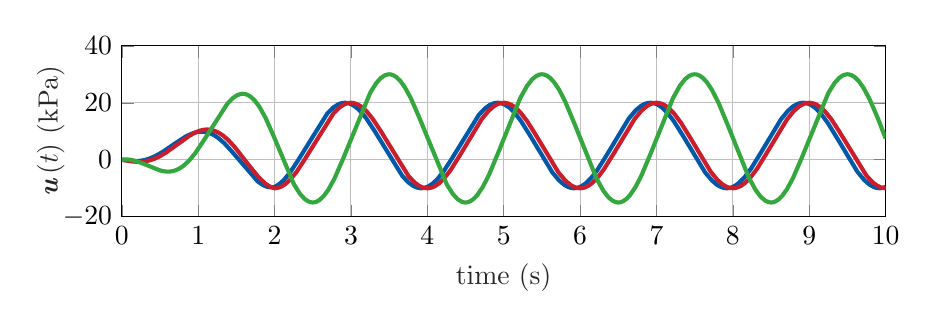
\begin{tikzpicture}

\begin{axis}[%
width=0.8\textwidth,
height=0.179\textwidth,
at={(0\textwidth,0\textwidth)},
scale only axis,
xmin=0,
xmax=10,
xlabel style={font=\color{white!15!black}},
xlabel={time (s)},
ymin=-20,
ymax=40,
ylabel style={font=\color{white!15!black}},
ylabel={$\textit{\textbf{u}}\,(t)$ (kPa)},
axis background/.style={fill=white},
xmajorgrids,
ymajorgrids,
ylabel style={yshift=-7.5pt}
]
\addplot [color=mycolor1, line width=1.5pt, forget plot]
  table[row sep=crcr]{%
0	-0\\
0.0800800800800801	-0.326421096773199\\
0.13013013013013	-0.446396146969825\\
0.16016016016016	-0.475915059812738\\
0.19019019019019	-0.468617984138909\\
0.22022022022022	-0.421114993853074\\
0.26026026026026	-0.290581235653967\\
0.31031031031031	-0.0133501719664331\\
0.37037037037037	0.490936189786673\\
0.44044044044044	1.30870274857828\\
0.53053053053053	2.67542755986546\\
0.67067067067067	5.2362166600556\\
0.830830830830831	8.06311411354436\\
0.910910910910911	9.10605922484043\\
0.970970970970971	9.61807923316933\\
1.01101101101101	9.80511023254271\\
1.04104104104104	9.85652001840668\\
1.06106106106106	9.8464167830638\\
1.08108108108108	9.79979543095045\\
1.11111111111111	9.65996707165884\\
1.15115115115115	9.34097577727256\\
1.2012012012012	8.72856335397239\\
1.26126126126126	7.68842452977073\\
1.34134134134134	5.82705175209153\\
1.44144144144144	2.89025349032573\\
1.78178178178178	-7.66126479630216\\
1.85185185185185	-8.93823786685945\\
1.9019019019019	-9.48537113895998\\
1.93193193193193	-9.65018897998966\\
1.95195195195195	-9.68800064376008\\
1.97197197197197	-9.66633786975596\\
1.99199199199199	-9.58391156057349\\
2.01201201201201	-9.38332861181659\\
2.06206206206206	-8.53932967412129\\
2.12212212212212	-7.08800557275741\\
2.2022022022022	-4.4965915337584\\
2.3023023023023	-0.439410784019138\\
2.69269269269269	16.3221257528725\\
2.77277277277277	18.415013753162\\
2.83283283283283	19.4356806473722\\
2.87287287287287	19.8329494125197\\
2.9029029029029	19.9772856135889\\
2.92292292292292	19.9995372186649\\
2.94294294294294	19.9624739715968\\
2.97297297297297	19.7960483764044\\
3.01301301301301	19.3698711750903\\
3.06306306306306	18.5189587240366\\
3.12312312312312	17.0600160253529\\
3.2032032032032	14.4600311678918\\
3.31331331331331	9.95268952377332\\
3.67367367367367	-5.71438002463892\\
3.75375375375375	-7.99033138710941\\
3.81381381381381	-9.16654342890359\\
3.86386386386386	-9.76383453862231\\
3.9039039039039	-9.97980651362566\\
3.92392392392392	-9.99909251603334\\
3.94394394394394	-9.95906542484922\\
3.97397397397397	-9.7882229857449\\
4.01401401401402	-9.35627162946138\\
4.06406406406407	-8.49845408003308\\
4.12412412412413	-7.03190721204662\\
4.20420420420421	-4.42337724832305\\
4.31431431431432	0.0918605166913373\\
4.67467467467468	15.7473395539602\\
4.75475475475476	18.0138529161429\\
4.81481481481482	19.1819782322969\\
4.86486486486487	19.7720990448672\\
4.8948948948949	19.9517886445088\\
4.91491491491492	19.9977546859628\\
4.93493493493494	19.9844129242011\\
4.95495495495496	19.9118161184931\\
4.98498498498499	19.692509501943\\
5.02502502502503	19.1973369064934\\
5.07507507507508	18.264138133125\\
5.14514514514515	16.4145743346791\\
5.22522522522523	13.6326840302821\\
5.34534534534535	8.50521702792188\\
5.63563563563564	-4.38647516760632\\
5.72572572572573	-7.28045577289802\\
5.7957957957958	-8.86491478632072\\
5.84584584584585	-9.59019275917794\\
5.88588588588589	-9.91179460555106\\
5.91591591591592	-9.99849667044506\\
5.93593593593594	-9.98218895327441\\
5.95595595595596	-9.90663498672929\\
5.98598598598599	-9.68293467832493\\
6.02602602602603	-9.18204294489704\\
6.07607607607608	-8.24204535487507\\
6.14614614614615	-6.38391405917885\\
6.22622622622623	-3.59406523774787\\
6.34634634634635	1.54066527788336\\
6.63663663663664	14.423222670133\\
6.72672672672673	17.3074818400554\\
6.7967967967968	18.8828466654283\\
6.84684684684685	19.6010714539438\\
6.88688688688689	19.9168288901412\\
6.91691691691692	19.9990903293176\\
6.93693693693694	19.979816818011\\
6.95695695695696	19.9013064378096\\
6.98698698698699	19.6732146498049\\
7.02702702702703	19.1666087318999\\
7.07707707707708	18.2198216212038\\
7.14714714714715	16.3531412039961\\
7.22722722722723	13.5553614553648\\
7.34734734734735	8.4134182056872\\
7.63763763763764	-4.45987698297003\\
7.72772772772773	-7.33438619403134\\
7.7977977977978	-8.90064125199644\\
7.84784784784785	-9.61180575338317\\
7.88788788788789	-9.92171565676419\\
7.91791791791792	-9.99953565670966\\
7.93793793793794	-9.97729654186992\\
7.95795795795796	-9.89583052442988\\
7.98798798798799	-9.66334951250793\\
8.02802802802803	-9.15103442013677\\
8.07807807807808	-8.19746715188983\\
8.14814814814815	-6.32225607345482\\
8.23823823823824	-3.12412058064418\\
8.35835835835836	2.09379127496054\\
8.62862862862863	14.1266639802227\\
8.71871871871872	17.0878879354425\\
8.78878878878879	18.7355625082257\\
8.84884884884885	19.6223955513405\\
8.88888888888889	19.926454857093\\
8.91891891891892	19.9998326482171\\
8.93893893893894	19.974628149775\\
8.95895895895896	19.8902073007435\\
8.98898898898899	19.6533393639939\\
9.02902902902903	19.1353201636276\\
9.07907907907908	18.1749821680047\\
9.14914914914915	16.2912589729894\\
9.23923923923924	13.0844270116058\\
9.35935935935936	7.85991719202451\\
9.62962962962963	-4.16405358395558\\
9.71971971971972	-7.1157584442214\\
9.78978978978979	-8.75445039392143\\
9.84984984984985	-9.63284074308951\\
9.88988988988989	-9.93104644425996\\
9.91991991991992	-9.99998130090296\\
9.92992992992993	-9.99330959530174\\
9.94994994994995	-9.93550877769289\\
9.97997997997998	-9.7382022827042\\
10	-9.53368632565967\\
};
\addplot [color=mycolor2, line width=1.5pt, forget plot]
  table[row sep=crcr]{%
0	-0\\
0.11011011011011	-0.501631548802106\\
0.17017017017017	-0.672771725604441\\
0.21021021021021	-0.719575951069583\\
0.24024024024024	-0.711925105415364\\
0.27027027027027	-0.663529844709625\\
0.31031031031031	-0.530499096325073\\
0.36036036036036	-0.247084664731663\\
0.42042042042042	0.270928243995186\\
0.49049049049049	1.1163420287873\\
0.58058058058058	2.54202613740464\\
0.71071071071071	5.05316960834889\\
0.890890890890891	8.52020306455763\\
0.970970970970971	9.67944745678268\\
1.03103103103103	10.2735946634854\\
1.07107107107107	10.5113084593509\\
1.1011011011011	10.5979484020371\\
1.12112112112112	10.6097926348153\\
1.14114114114114	10.5837544842323\\
1.17117117117117	10.4719971670263\\
1.21121121121121	10.184624855263\\
1.26126126126126	9.60122488058117\\
1.32132132132132	8.57852016935115\\
1.39139139139139	6.97040405862983\\
1.48148148148148	4.34975735826455\\
1.63163163163163	-0.838417883808095\\
1.79179179179179	-6.18516552979148\\
1.88188188188188	-8.44875503362838\\
1.94194194194194	-9.46811471757773\\
1.99199199199199	-9.95523231675877\\
2.002002002002	-9.99970331978025\\
2.02202202202202	-9.96411589164284\\
2.05205205205205	-9.79989003331738\\
2.09209209209209	-9.37658932472964\\
2.14214214214214	-8.52911802342114\\
2.2022022022022	-7.07396678042702\\
2.28228228228228	-4.4782460740071\\
2.38238238238238	-0.417331272446525\\
2.77277277277277	16.3376476120192\\
2.85285285285285	18.425593622457\\
2.91291291291291	19.4420981038878\\
2.95295295295295	19.8364558610294\\
2.98298298298298	19.9785698881821\\
3.003003003003	19.9993324722562\\
3.02302302302302	19.9607810138446\\
3.05305305305305	19.7921374866907\\
3.09309309309309	19.3630605175579\\
3.14314314314314	18.5086799195633\\
3.2032032032032	17.0459173142334\\
3.28328328328328	14.4416386890202\\
3.39339339339339	9.93032677916854\\
3.75375375375375	-5.73094246460772\\
3.83383383383383	-8.00215775878589\\
3.89389389389389	-9.17431085668792\\
3.94394394394394	-9.76800245162413\\
3.97397397397397	-9.94988880393029\\
3.99399399399399	-9.9973299484371\\
4.01401401401402	-9.98546496932957\\
4.03403403403404	-9.91434078602069\\
4.06406406406407	-9.69722257406094\\
4.10410410410411	-9.20489933310494\\
4.15415415415416	-8.27508909582531\\
4.22422422422423	-6.42979782943817\\
4.30430430430431	-3.65188028723395\\
4.42442442442443	1.47195134180766\\
4.71471471471472	14.3681441665571\\
4.80480480480481	17.2669543507487\\
4.87487487487488	18.8559354690983\\
4.92492492492493	19.5847225103823\\
4.96496496496497	19.9092330715828\\
4.994994994995	19.9981457807168\\
5.01501501501502	19.983314776841\\
5.03503503503504	19.9092330715828\\
5.06506506506507	19.6877200825019\\
5.10510510510511	19.1896752583361\\
5.15515515515516	18.2530616010562\\
5.22522522522523	16.3991937198305\\
5.30530530530531	13.6133039531094\\
5.42542542542543	8.48218355487591\\
5.71571571571572	-4.40493793222117\\
5.80580580580581	-7.29404091858868\\
5.87587587587588	-8.87393563930486\\
5.92592592592593	-9.59567305869735\\
5.96596596596597	-9.91434078602069\\
5.995995995996	-9.99881329085688\\
6.01601601601602	-9.98101640888201\\
6.03603603603604	-9.90397791429554\\
6.06606606606607	-9.67807233871631\\
6.10610610610611	-9.17431085668794\\
6.15615615615616	-8.23090304192219\\
6.22622622622623	-6.36847687943411\\
6.30630630630631	-3.57464243887714\\
6.42642642642643	1.56371598502504\\
6.71671671671672	14.4416386890202\\
6.80680680680681	17.3210059061694\\
6.87687687687688	18.8917986050964\\
6.92692692692693	19.6064792650725\\
6.96696696696697	19.9193010070972\\
6.996996996997	19.9993324722562\\
7.01701701701702	19.9785698881821\\
7.03703703703704	19.8985753661291\\
7.06706706706707	19.6682794381143\\
7.10710710710711	19.1588062801045\\
7.15715715715716	18.2086136375572\\
7.22722722722723	16.3376476120192\\
7.31731731731732	13.1438538385475\\
7.43743743743744	7.92924631633511\\
7.70770770770771	-4.10801423849995\\
7.7977977977978	-7.07396678042701\\
7.86786786786787	-8.72610767741176\\
7.92792792792793	-9.61714102264125\\
7.96796796796797	-9.92411368575894\\
7.997997997998	-9.99970331978025\\
8.01801801801802	-9.97597523893575\\
8.03803803803804	-9.89302548051136\\
8.06806806806807	-9.65834147754138\\
8.10810810810811	-9.14316168191625\\
8.15815815815816	-8.18619360838943\\
8.22822822822823	-6.30670622246757\\
8.31831831831832	-3.10420022249363\\
8.43843843843844	2.11703096413143\\
8.70870870870871	14.1454488268896\\
8.7987987987988	17.1018968427548\\
8.86886886886887	18.7450632184755\\
8.92892892892893	19.6276582259656\\
8.96896896896897	19.9287787744115\\
8.998998998999	19.9999258297617\\
9.00900900900901	19.9939926067748\\
9.02902902902903	19.9376659986101\\
9.05905905905906	19.7425530097099\\
9.0990990990991	19.2789095829369\\
9.14914914914915	18.3832530253536\\
9.20920920920921	16.8751286521203\\
9.28928928928929	14.2200463063114\\
9.3993993993994	9.66216405538659\\
9.74974974974975	-5.59825969650894\\
9.82982982982983	-7.9070465162216\\
9.88988988988989	-9.11145304096914\\
9.93993993993994	-9.73377816012621\\
9.97997997997998	-9.97034165890616\\
10	-10\\
};
\addplot [color=mycolor3, line width=1.5pt, forget plot]
  table[row sep=crcr]{%
0	0\\
0.03003003003003	0.0807875327721987\\
0.05005005005005	0.0995177754531404\\
0.0800800800800801	0.0760358368166152\\
0.11011011011011	-0.00709801900616824\\
0.15015015015015	-0.204522657283015\\
0.2002002002002	-0.574235657359171\\
0.28028028028028	-1.38026403403502\\
0.5005005005005	-3.75374679332919\\
0.55055055055055	-4.05118950526915\\
0.59059059059059	-4.16216470722652\\
0.61061061061061	-4.16899215652725\\
0.63063063063063	-4.14063717490415\\
0.66066066066066	-4.02816705458735\\
0.7007007007007	-3.73954347430554\\
0.75075075075075	-3.14276802206605\\
0.810810810810811	-2.0673375762551\\
0.880880880880881	-0.319265372442111\\
0.960960960960961	2.28103577248515\\
1.07107107107107	6.6845980546254\\
1.38138138138138	19.6541002190833\\
1.45145145145145	21.582216776485\\
1.51151151151151	22.6615540471951\\
1.55155155155155	23.0448593918814\\
1.58158158158158	23.1425319046665\\
1.6016016016016	23.1139274538405\\
1.62162162162162	23.0087863087877\\
1.65165165165165	22.7055645267611\\
1.69169169169169	22.0273798665317\\
1.74174174174174	20.7417666423772\\
1.8018018018018	18.5783053487758\\
1.88188188188188	14.7341728443266\\
1.98198198198198	8.69390312369267\\
2.25225225225225	-8.52207642219807\\
2.33233233233233	-11.950096997847\\
2.39239239239239	-13.7265022111106\\
2.44244244244244	-14.6331628390412\\
2.48248248248248	-14.9659366170868\\
2.5025025025025	-14.9993046570243\\
2.52252252252252	-14.9437004233762\\
2.55255255255255	-14.6940480756536\\
2.59259259259259	-14.0547640270985\\
2.64264264264264	-12.7783735247838\\
2.7027027027027	-10.5899354332562\\
2.78278278278278	-6.68993111345754\\
2.89289289289289	0.0711063659811551\\
3.25325325325325	23.571674319608\\
3.33333333333333	26.9855715851499\\
3.39339339339339	28.7498641210686\\
3.44344344344344	29.6457781447508\\
3.48348348348348	29.9697174992203\\
3.5035035035035	29.9986371345066\\
3.52352352352352	29.9385871358887\\
3.55355355355355	29.6823095275664\\
3.59359359359359	29.0343642599611\\
3.64364364364364	27.7476161367747\\
3.7037037037037	25.5477718369885\\
3.78378378378378	21.634949939152\\
3.89389389389389	14.8620684192999\\
4.25425425425426	-8.62111327836262\\
4.33433433433434	-12.020853472521\\
4.3943943943944	-13.7730158833619\\
4.44444444444445	-14.6581744427747\\
4.47447447447448	-14.9276949035333\\
4.4944944944945	-14.9966346065618\\
4.51451451451452	-14.9766125945736\\
4.53453453453454	-14.8677080435236\\
4.56456456456457	-14.5387342360751\\
4.60460460460461	-13.7959572690342\\
4.65465465465466	-12.3961376176975\\
4.72472472472473	-9.62176482738752\\
4.80480480480481	-5.44890418732252\\
4.92492492492493	2.24231934080432\\
5.21521521521522	21.5798289791656\\
5.30530530530531	25.9207692232311\\
5.37537537537538	28.2974290404894\\
5.42542542542543	29.3853237308211\\
5.46546546546547	29.8677080435236\\
5.4954954954955	29.9977471147519\\
5.51551551551552	29.9732761701136\\
5.53553553553554	29.859935880122\\
5.56556556556557	29.5243715418119\\
5.60560560560561	28.7730158833619\\
5.65565565565566	27.3629980363039\\
5.72572572572573	24.575774058032\\
5.80580580580581	20.3909757294455\\
5.92592592592593	12.6888570917049\\
6.21621621621622	-6.63494993915191\\
6.30630630630631	-10.9613079399095\\
6.37637637637638	-13.3243264257378\\
6.42642642642643	-14.4016413170101\\
6.46646646646647	-14.8752590044937\\
6.4964964964965	-14.9986371345066\\
6.51651651651652	-14.9697174992203\\
6.53653653653654	-14.8519425911507\\
6.56656656656657	-14.5097910404972\\
6.60660660660661	-13.7498641210687\\
6.65665665665666	-12.3296620224706\\
6.72672672672673	-9.52961442011234\\
6.80680680680681	-5.33291978800277\\
6.92692692692693	2.38001779028815\\
7.21721721721722	21.6899311134575\\
7.30730730730731	26.0016640859732\\
7.37737737737738	28.3510178716189\\
7.42742742742743	29.4177423098716\\
7.46746746746747	29.8825886883582\\
7.4974974974975	29.9993046570243\\
7.51751751751752	29.9659366170868\\
7.53753753753754	29.8437282556583\\
7.56756756756757	29.4949928763229\\
7.60760760760761	28.7265022111106\\
7.65765765765766	27.2961299058697\\
7.72772772772773	24.483286370118\\
7.81781781781782	19.6860556098343\\
7.93793793793794	11.8591669028303\\
8.20820820820821	-6.19011422236993\\
8.2982982982983	-10.6319201315475\\
8.36836836836837	-13.1034036412538\\
8.42842842842843	-14.433626550177\\
8.46846846846847	-14.889697022631\\
8.4984984984985	-14.9997496757036\\
8.50850850850851	-14.9919622724002\\
8.52852852852853	-14.9096932358798\\
8.55855855855856	-14.6203286504033\\
8.5985985985986	-13.9291751149002\\
8.64864864864865	-12.5908318083653\\
8.70870870870871	-10.3342850416879\\
8.78878878878879	-6.35795820526154\\
8.8988988988989	0.473136504791515\\
9.24924924924925	23.3723340107839\\
9.32932932932933	26.8425205540668\\
9.38938938938939	28.6551579159696\\
9.43943943943944	29.5940041341939\\
9.47947947947948	29.9532610881355\\
9.4994994994995	29.9999721861434\\
9.50950950950951	29.9899599424897\\
9.52952952952953	29.9032493634039\\
9.55955955955956	29.6072757057591\\
9.5995995995996	28.9075006803715\\
9.64964964964965	27.5588776357114\\
9.70970970970971	25.2910568755896\\
9.78978978978979	21.3021465209999\\
9.8998998998999	14.4596113812496\\
10	7.50000000000003\\
};
\end{axis}
\end{tikzpicture}%
  \fi
  \caption{(top) Soft robot manipulator with three parallel embedded pneumatic bellows. This manipulator changes its pose by inflation or deflation of the parallel pneumatic channels (<0.1 \si{\mega \pascal}). (bottom) Differential pressure signals applied on the internal bellows structures given by the input vector $\uB = (u_1\,u_2,\,u_3)^\top$, shown by the trajectories (\ldata{Matlab1},\ldata{Matlab2},\ldata{Matlab3}), respectively.}
  \vspace{-0.1cm}
  \label{fig:C2:soft_robot}
\end{figure}
%

\begin{rmk}[Additive manufacturing] The soft robot is exclusively composed of a printable, flexible thermoplastic elastomer (Young's modulus $\le$ 80 \si{\mega \pascal}), which intrinsically promotes softness and dexterity. The elastomer material is developed explicitly for Selective Laser Sintering (SLS), a 3-Dimensional (3D) printing method that uses a laser to solidify powdered material. The main advantage of SLS printing over other techniques is that the printed parts are fully self-supported, which allows for highly complex and high-detail structures. It should be mentioned, though, that the layer-by-layer material deposition will introduce undesired anisotropic mechanical effects. To mitigate anisotropy, the bellows are printed orthogonal to the printing plane, thereby ensuring mechanical symmetry. For the majority of this work, the 3D-printed soft robot in Figure \ref{fig:C2:soft_robot} will form the basis of the dynamical model. The 3D model is made available at the open repository \cite{Caasenbrood2020}.
\end{rmk}
